\documentclass[11pt, a4paper, twoside]{Thesis}

\usepackage{subcaption}
\usepackage{amsmath}
\usepackage{tocbibind}
\usepackage{multirow}
\usepackage{setspace}
\usepackage{todonotes}
\usepackage{packages/algorithm2e}
\usepackage{textcomp}

\setlength{\parindent}{0.7cm}

\makeatletter
\DeclareRobustCommand\onedot{\futurelet\@let@token\@onedot}
\def\@onedot{\ifx\@let@token.\else.\null\fi\xspace}

\def\eg{\emph{e.g}\onedot} \def\Eg{\emph{E.g}\onedot}
\def\ie{\emph{i.e}\onedot} \def\Ie{\emph{I.e}\onedot}
\def\cf{\emph{c.f}\onedot} \def\Cf{\emph{C.f}\onedot}
\def\etc{\emph{etc}\onedot} \def\vs{\emph{vs}\onedot}
\def\wrt{w.r.t\onedot} \def\dof{d.o.f\onedot}
\def\etal{\emph{et al}\onedot}
\makeatother

\newcommand{\argmax}{\operatornamewithlimits{argmax}}
\newcommand{\argmin}{\operatornamewithlimits{argmin}}
\newcommand{\abs}[1]{\left\lvert#1\right\rvert}
\newcommand{\norm}[1]{\left\lVert#1\right\rVert}
\newcommand{\listofalgorithmes}{\tocfile{\listalgorithmcfname}{loa}}

\begin{document}
% *************** Front matter ***************
\frontmatter

\title  {Rendering and Streaming of
Bidirectional Texture Functions }

\authors  {\texorpdfstring
            {{Oleksandr Sotnychenko}}
            {Oleksandr Sotnychenko}
            }
\addresses  {\groupname\\\deptname\\\univname}  % Do not change this here, instead these must be set in the "Thesis.cls" file, please look through it instead
%\usdate
\date       {Saarbr\"ucken, \today }
\subject    {}
\keywords   {}

\maketitle

%\newpage
%\mbox{}
%\thispagestyle{empty}
%\newpage

\setstretch{1.3}

\thispagestyle{empty}

\section*{Eidesstattliche Erkl\"{a}rung}
Ich erkl\"{a}re hiermit an Eides Statt, dass ich die vorliegende Arbeit selbstst\"{a}ndig verfasst und keine
anderen als die angegebenen Quellen und Hilfsmittel verwendet habe.

\vspace{0.60cm}
\section*{Statement in Lieu of an Oath}
I hereby confirm that I have written this thesis on my own and that I have not used any other media or
materials than the ones referred to in this thesis.
\vspace{1.5cm}

\section*{Sperrvermerk}


\vspace{0.60cm}
\section*{Blocking Notice}

\vspace{3cm}

\begin{flushright}
\noindent Saarbr\"{u}cken, \today
\hfill
Oleksandr Sotnychenko
\end{flushright}

\clearpage  % Declaration ended, now start a new page
%% ----------------------------------------------------------------

\newpage
\mbox{}
\thispagestyle{empty}
\newpage

% The Abstract Page
\addtotoc{Abstract}  % Add the "Abstract" page entry to the Contents
\abstract{
\addtocontents{toc}{\vspace{1em}}  % Add a gap in the Contents, for aesthetics

Bidirectional Texture Function (BTF) is a 6-dimensional function that depends on spatial position on a texture surface and on light and camera views.
An appearance of realistic materials drastically changes with light and camera variations.
 BTF can model reliable presentation of such materials and capture reflectance properties with a wide range of illumination variations.

In this work we present WebGL-based rendering of BTF in a web-browser. 
An ever-growing number of mobile devices that use web-browser implies that rendering must be possible for hardware with very limited capabilities.
Also, due to enormous size of BTF - compression step is inevitable. 
We employ a principal component analysis to compress the data, which allows for rendering of BTF with interactive frame rates. 
To provide immediate feedback to the user we provide a solution to stream the BTF data and to progressively enhance the rendering quality while the data downloads. 






}
\clearpage
%% ----------------------------------------------------------------
\newpage
\mbox{}
\thispagestyle{empty}
\newpage

\setstretch{1.3}  % Reset the line-spacing to 1.3 for body text (if it has changed)

% The Acknowledgements page, for thanking everyone
\acknowledgements{
\addtocontents{toc}{}  % Add a gap in the Contents, for aesthetics    \vspace{1em}


I am deeply grateful to my adviser Jan Sutter for giving me motivation, for sharing his experience with me and for his continuous support in writing my thesis.
I am thankful to my supervisor Prof. Dr. Philipp Slusallek for inspiring me to write the thesis in the field of Computer Graphics and providing me with valuable pieces of advice.
Special thanks go to Kristian Sons and Felix Klein for giving me a continues support and for providing me with directions.

I would like to express my sincere gratitude to Saarland University for providing excellent studying possibilities. 
I am thankful to the German Research Center for Artificial Intelligence for very pleasant working atmosphere.

 Last but not least, I am especially thankful for my parents and friends, who supported me during my studies.






}
\clearpage  % End of the Acknowledgements
%% ----------------------------------------------------------------
\newpage
\mbox{}
\thispagestyle{empty}
\newpage

\thispagestyle{empty}
\emph{To my family.}
\clearpage

\newpage
\mbox{}
\thispagestyle{empty}
\newpage

\setstretch{1}
\begin{spacing}{0.1}
\pagestyle{fancy}
\tableofcontents
\newpage
\listoffigures
\newpage
%\listoftables
%\newpage
%\listofalgorithmes
\end{spacing}

\clearpage

\setstretch{1.3}
% *************** Main matter ***************
\mainmatter

\chapter{Introduction}
\label{chapter:introduction}

One of the main goals in computer graphics is realistic rendering. 
Even though computer graphics is constantly improving, we are still quite away from reality because material representation in a traditional way lack important realistic properties. 
A 2-D texture in conjunction with a shading model is a conventional way to represent material appearances in rendering.
Real-world materials surfaces on the other hand consist of surface meso-structures, i.e. intermediate in between micro and macro structures.
Meso-structures are responsible for fine-scale shadows, self-occlusions, inter-reflection, subsurface scattering and specularities.
Also, reflectance and the look of real-world materials can drastically change when camera and light directions vary.

One of the possible solution to represent such material attributes is to use sophisticated light functions, for instance a Bidirectional Texture Function (BTF). 
 A BTF is a 6-dimensional function that depends on camera and light directions as well as on spatial texture coordinates. 
The BTF conceptually extends traditional 2-D textures by the dependence on light and camera directions.
This function is usually acquired as a data-set of thousands of images that cover discrete light and camera directions.
Due to the enormous size of that data direct renderings even on modern hardware without any compression is impractical.
Fortunately, many techniques exist to deal with the huge size of BTFs, i.e. compression methods.


In this thesis, we use \emph{WebGL} for real-time rendering of BTF in the Web.
Even though 3-D graphics for the Web becoming more and more popular. BTFs are rarely used realistic rendering, due to their huge size and the overall computational effort needed for rendering,
including decompression of the data and interpolation of camera and light directions.
Such demanding computational effort is time consuming, especially for on mobile-devices.

And the problem which arises when rendering BTFs in a Browser is the transmission of the data.
Before rendering on the client side, the transmission of the data has to be finished.
Even the transfer of a compressed BTF data can take a considerable amount of time. 
The compressed BTF can be tens of megabytes in size.
Because users are eager to see a result, especially on the Web, we use a streaming solution to deliver the data as quickly as possibly, while steadily increasing the resulting image.
 \emph{Web-Sockets} are the state of the art technique for streaming and are supported by most of today's browsers.
With \emph{Web-Sockets}  a  full-duplex communication is available for the server and the client, which is faster than traditional HTTP-based methods. 
This promises fast and reliable solution for real-time performance in \emph{WebGL}-based application.

In this thesis we use a PCA for compression, which allows for a considerably good compression ratio with low decompression error.
Also, it is well suited for real-time rendering and streaming.

We implemented WebGL demo web-application and \emph{Web-Sockets} server for streaming purposes.



\section{Related Work}
\label{section:related_work}

Nowadays, Web technologies are able to support WebGL \cite{webgl}, which is a JavaScript API for rendering 3D content.
WebGL provides  vertex and fragment shaders  for creating highly realistic rendering results.
New standards for 3D graphics in context of HTML domain are evolving, for instance such as XML3D \cite{xml3d}.
XML3D allows for embedding 3D graphics into HTML pages. XML3D is based both on XML and WebGL.
It allows for declaring 3D scenes elements in the context of HTML pages.
Web programmers can apply their existing knowledge (i.e. about DOM, XML, CSS) to include 3D graphics in the HTML content by using XML3D.
Currently XML3D  natively supported by  Firefox and Google Chrome browsers on Linux and Windows.
 
Most of previous work that used BTFs for realistic rendering were primarily intended  for offline applications.
However, their approach is not suitable in the context of the Web, due to the data transfer between the server and a client.
  Schwartz \emph{et. al.} \cite{webglbtfstreaming} presented a work in which compressed BTF data is streamed from the server to a client.
 The streaming over the Internet is done by means of HTTP streaming, i.e. the web-application requests the data in small chunks.
 With each new chunk of the BTF data the rendering quality of the 3D object is progressively enhanced.
 We on the other hand, use \emph{Web-Sockets} to improve application performance compared to HTPP streaming, by reducing the network latency and streaming the data in a binary form.

 
Existing BTF compression methods are reviewed by Haindl \emph{et. al.} \cite{haindl, haindl_visual}.
A trade-off has to be made between the rendering quality and compression rate depending on the intended application.
 Our compression method is related to the PCA RF (Principal Component Analysis Reflectance Field) method, which was introduced by Sattler \emph{et. al.} \cite{star2004}.
This method allows for real-time performance with realistic rendering quality. 
Sattler performs PCA on each of the $n$ camera directions separately. We on the other hand, perform PCA on $k$ neighbour camera directions at once.
In Haindl's review \cite{haindl} PCA based methods achieve better or at least equal reconstruction results than most other methods.
Compression rates of PCA methods are not as high as those of other methods. However, those methods, which produce better compression rates, have worse quality than PCA based methods.



\section{Outline}
\label{section:outline}

\begin{figure}[h]
 \centering
 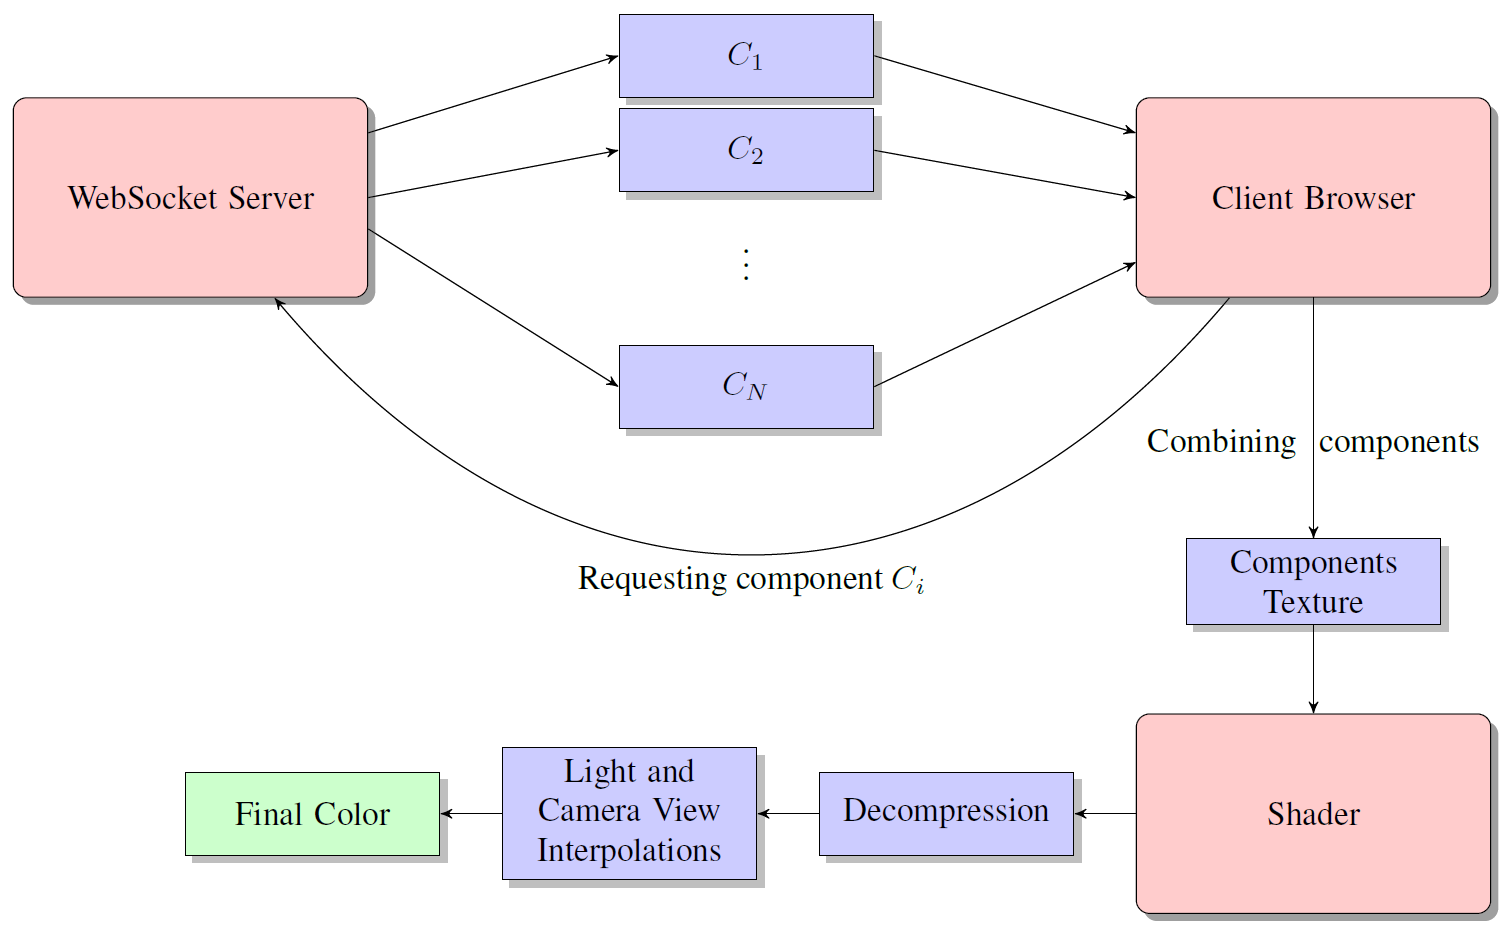
\includegraphics[width=1.0\textwidth]{figures/overview}
 \caption[Model Overview ] {
 	{\bf Model Overview}

	
	}
 \label{fig:overview}
\end{figure}




\clearpage



\chapter{Methods}
\label{chapter:solutions}


This Chapter has the following structure. Section \ref{section:acquisition}
describes methods of BTF acquisition and reviews some of the publicly available BTF datasets.
 Section \ref{section:compression_and_decompression} argues about the choice of compression methods, while
  Section \ref{section:pca} defines our chosen compression method.
 Section \ref{section:interpolation} defines a solution for viewing and illumination angle interpolation.
The last Section \ref{section:streaming}
concludes the Chapter with proposing our web-socket streaming model. 

\section{BTF Acquisition}
\label{section:acquisition}

BTF acquisition is not a trivial task, since to get an accurate and reliable BTF data, it is required to have an efficient BTF measurement system. 
A pioneer in this task were Dana et. al. \cite{curetDataBase}, who measured 61 materials with fixed light and moving around camera that photographed a flat surface of a material.
Such procedure results in a set of images, i.e. BTF, which can be regarded as a 6D reflectance field function \cite{sattler-2003-efficient} 

{\centering $L=L(x,y,\theta _{i},\phi _{i},\theta _{o},\phi _{o})$ \\}


where $(x,y)$ is a surface point of a flat sampled material, $(\theta _{i},\phi _{i})$ incoming light direction (light direction) and $(\theta _{o},\phi _{o})$ outgoing light direction (camera direction).

For each measured surface Dana et. al. used 205 different combinations of viewing and illumination directions. The resulted BTF can be gigabytes in size. To achive reasonable real-time performance compression of BTF
is an inevitable step. Also, Dana's et. al. BTF database is not spatially registered, i.e. images were not mutually registered for different view angles. That means one should further process the database in order to render BTF.

Based on Dana et. al. BTF measurement system, Sattler from Bonn University made his own measuring system \cite{sattler-2003-efficient}. The main difference in that system is that a camera moves on a semi-circle rail around a material.
Also, such setup provides spatially registered data, with reasonable angular and spatial resolutions. Datasets of Bonn University \cite{btfBonn} are publicly available and were used in this thesis.



\begin{figure}[h]
 \centering
 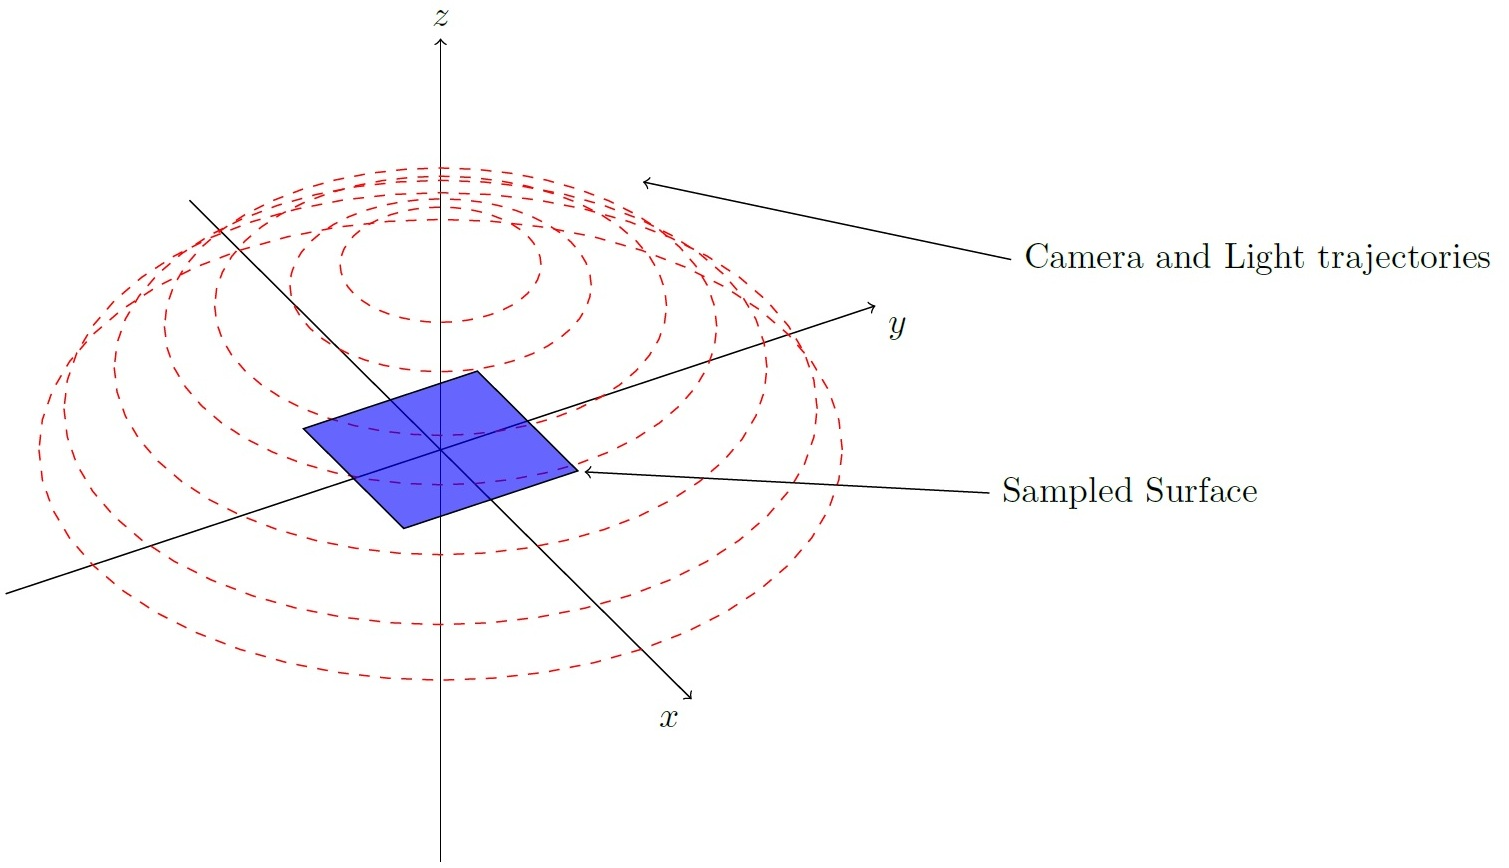
\includegraphics[width=1.0\textwidth]{figures/acquisition}
 \caption[Example of BTF measurement] {
 	{\bf Example of BTF measurement.}

	Camera and light positions share the same trajectories.
	Red dashed circles are the sample positions on the hemisphere. }
 \label{fig:acquisition_example}
\end{figure}


 Consider Figure \ref{fig:acquisition_example}, which illustrates one of the possible ways of sampling the material.
The measured surface is being fixed all the time on the sampler holder. Then, for each light position, a camera photographs the flat material while moving from point to point of the hemisphere.
Bonn database has the same trajectory for camera and light positions, i.e. 81 positions on the hemisphere, which results in 6561 total number of acquired images.



\begin{figure}[h]
 \centering
 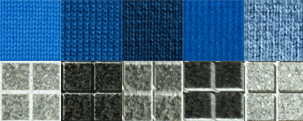
\includegraphics[width=1.0\textwidth]{figures/exampleBTF}
 \caption[Example of BTF measurement] {
 	{\bf BTF example of Bonn Database \cite{btfBonn}.}

	Example how BTF catches rich appearance of the material due to dependencies on light and camera views. 
	Upper row is a knitted wool, lower is a graved granite stone.}
 \label{fig:exampleBTF}
\end{figure}



\section{Compression and Decompression}
\label{section:compression_and_decompression}

As we already know BTF is a high dimensional data, which makes it enormous in size.
Datasets of Bonn are 8-bit PNG images with $256\times256$ resolution.
 Then, after an uncompressed PNG data loads to GPU it occupies approx. 1,2 GB of space. And that's not even large a spatial resolution in this case!
 Therefore, it is impractical to render BTF as a raw data even on the most modern GPUs.
 
 The most common technique to compress BTF is Principal component analysis (PCA), which is widely used in image compression \cite[Ch.\ 15]{haindl,gpu_gems}.
 PCA were used in several works of Bonn University \cite{sattler-2003-efficient,mueller-2003-compression,mueller-2004-environmental}.
 Also, at some point PCA were employed as a basis for Decorrelated Full Matrix Factorization compression method \cite{webglbtfstreaming}.
 
 The reason that PCA is the broadly used is because a user can straightforwardly change parameters of the model and control a trade between compression ratio and a reconstructed image quality.
 Unlikely, other methods based on probabilistic MRF models \cite{haindl}, even though probabilistic  methods provide thousand times better compression rate than linear factorization methods.
 Also, one more advantage of PCA is that is more suitable for low-end GPUs, because for example MRF methods can be very heavy for GPU.
 
 
\subsection{PCA}
\label{section:pca}

By a common definition Principal component analysis (PCA) is a mathematical tool that reduces the dimensions of possibly correlated variables. New reduced dimensions are called \emph{principal components}.
Principal components hold the most important variations of the data, e.g. first ones hold the biggest amount of texture details. Using principal components it is possible to reconstruct the whole data. 
Due to neglecting small variations of the variables at first place, the reconstructed data will differ from original one, but the most important variations of the data will be preserved. 
That's why PCA is good for image compression, because a human eye is not that sensitive to small variations, i.e. reconstructed image might look almost the same as original for an observer.
The good part about losing small variations, is that we can reduce some noise that was present in the original images \cite{pca_noise}.
\subsection{Data representation}
\label{section:first_step}

First step in our analysis is to chose a suitable data representation. Basically, there are two common arrangements, i.e. as a set of images or BRDFs (Bidirectional reflectance distribution function). 
Both representations can be mathematically interpreted as  \cite{mueller-2003-compression}


{\centering $\,\,BTF_{BRDF} \;\, = \left \{ {P_{(x)}} \right \}_{(x)\in I\subset \mathbb{N}^{2}}$ \\}
{\centering $BTF_{Image}=\left \{ I_{(v,l)} \right \}_{(v,l)\in M}$\\}

where $M$ denotes a set of images $I_{(v,l)}$ measured for different view and light directions $(v,l)$ accordingly.
$BTF_{BRDF}$ denotes a set of $P_{(x)}$ images, where each of them depends on a single spatial position $x$ for all possible views, i.e. $ \forall (v,l):x \in I_{(v,l)}$.
Note that such BRDFs are not fulfilling physical demanded property such as reciprocity, because they already contain a factor between an incident light direction and a normal, i.e. $n*l$.
In our case with Bonn datasets the sizes of variable vectors which we want to compress are $\left | I \right | = 3\times256\times256$ and $\left | M \right | = 3\times81\times81$, where $3$ stands for RGB channels.


M{\"u}ller et. al. \cite{mueller-2003-compression, haindl} claim that BRDF representation works slightly better in comparison to image-wise. 
The advantage of BRDF is that a compression ratio can be 10 times better and reconstruction error is slightly smaller than the image-wise representation.
Also, Borshukov et. al. \cite[Ch.\ 15]{gpu_gems} chose BRDF representation, claiming that it provides better compression ratio.
The reason why BRDF provides better compression ratio is because it provides better pixel-to-pixel comparison than image-wise. 
Each variable vector of BRDF arrangement depends only on a surface complexity \cite{mueller-2003-compression}, i.e. 
on a variation of reflection properties at a spatial point of the surface.
On the contrary, image-wise variable depends on the whole measured image plane, thus it is logical that it may provide lower compression rate due to stronger variations.
After all, we have chosen BRDF data representation based on such reasons, with which we have achieved $1:100$ compression ratio. 

\subsection{Algorithm}
\label{section:algorithm_step}
The algorithm of PCA for BTF compression and decompression is mainly borrowed from  Borshukov et. al \cite[Ch.\ 15]{gpu_gems}.
 Basically, this is a common algorithm of PCA that deploys computing a singular value decomposition (SVD).

In the \emph{first} step of algorithm we built BRDF representation of the BTF data.
Let matrix $A$ denote the stored BTF data.
We consider each image $I$ as three column vectors $a_{i}$ (red, green, and blue channels), where $i=0..3*N$. $N$ is the number of images.
The size of $a_{i}$ is $W\times H$, where $W$ and $H$ are dimensions of the image.
So, matrix $A$ has the following dimensions $(W*H)\times(3*N)$, which consist of such columns $a_{i}$.
Rows of matrix $A$ are BRDF representation of BTF, which will be dimensionally reduced.

The  \emph{second} step is called "centring" of the data. We compute the average value of each row of matrix $A$

{\centering $m_i=\frac{1}{3N}\sum_{i=1}^{3N}A_{i,j}$ \\}

Then, we subtract mean vector from each column of matrix $A$

{\centering $B_{i,j}=A_{i,j}-m_i.$ \\}

At the \emph{last} step, we compute singular value decomposition (SVD) of matrix $B$. The result of which will be such decomposition

{\centering $B=U\Sigma V^{T}$ \\}

where matrix $U$ holds \emph{principal components} of size $W\times H$. $\Sigma$ is a diagonal matrix and holds the "importance" value of each principal components, and
matrix $V$ stores weights that are needed for reconstructing matrix $B$.

\subsection{Compression}
\label{section:compression}




\begin{figure}[h]
 \centering
 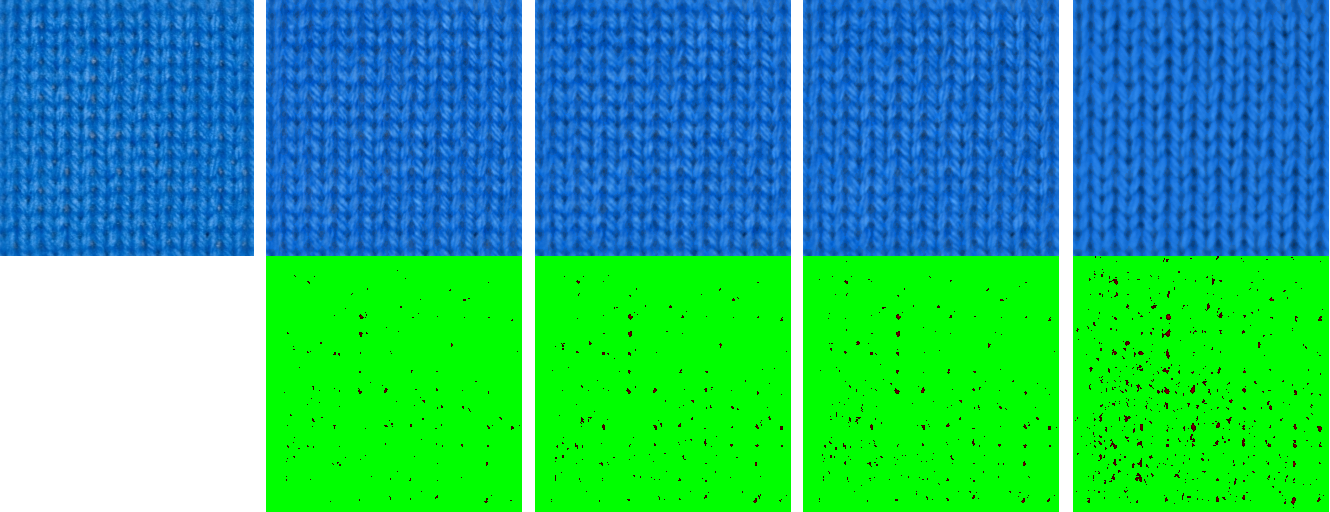
\includegraphics[width=1.0\textwidth]{figures/differ0}
 \caption[Example of compression ] {
 	{\bf Example of compression \textnumero 1.}

	\textbf{First row} from the left to the right: original image, \textbf{32} components (RMSE:7.7\%), \textbf{16} components (RMSE:8.2\%), \textbf{8} components (RMSE:8.5\%), \textbf{4} components (RMSE:10\%). 
	
	\textbf{Second row}: the difference between original and decompressed, \emph{red} color denotes how big the error, \emph{green} denotes that error is absent or very small.}
 \label{fig:compression_example_1}
\end{figure}



In order to achieve good compression ratio and at the same time preserve a decompressed quality we need to chose suitable parameters for PCA.
We perform PCA on subsets of 81 camera views. For each camera view there are 81 images sampled for different light directions.
We take $3$ neighbour views at once and perfrom PCA on them. With such size of subset we can achieve good trade between quality and compression ratio.
 For subsets of size $1$ RMSE (Root mean square error) improves to 5\%-7\% on average.
If we want to achieve even bigger compression ratio we can make the size of the subset even bigger, but of course the quality of decompressed texture will be worse compared to smaller subset sizes.
Also, performing PCA on the bigger subsets is inefficient, e.g. the time required to perform PCA on all $81$ views at once can take hours and memory requirements to compute SVD are demanding.


Consider examples  shown in Figure \ref{fig:compression_example_1}. We can see that for $4$ components all images are getting blurred.
In our case, $8$ components is a reasonable choice, as even for $32$ components the quality improvement is not that visible. Besides, smaller number of components will make decompression performance better.


The second example in Figure \ref{fig:compression_example_2} has worse reconstructed quality than in Figure \ref{fig:compression_example_1} due to small specularities on the surface, which are not preserved in principal components.
This example demonstrates the limitation of PCA, i.e. such small details may not be reconstructed.
But, an overall structure and a tone of the texture is preserved.
Also, compression ration 1:100 is achieved with such parameters, i.e. from 1,2 GB we now store around 20 MB in GPU.




\begin{figure}[h]
 \centering
 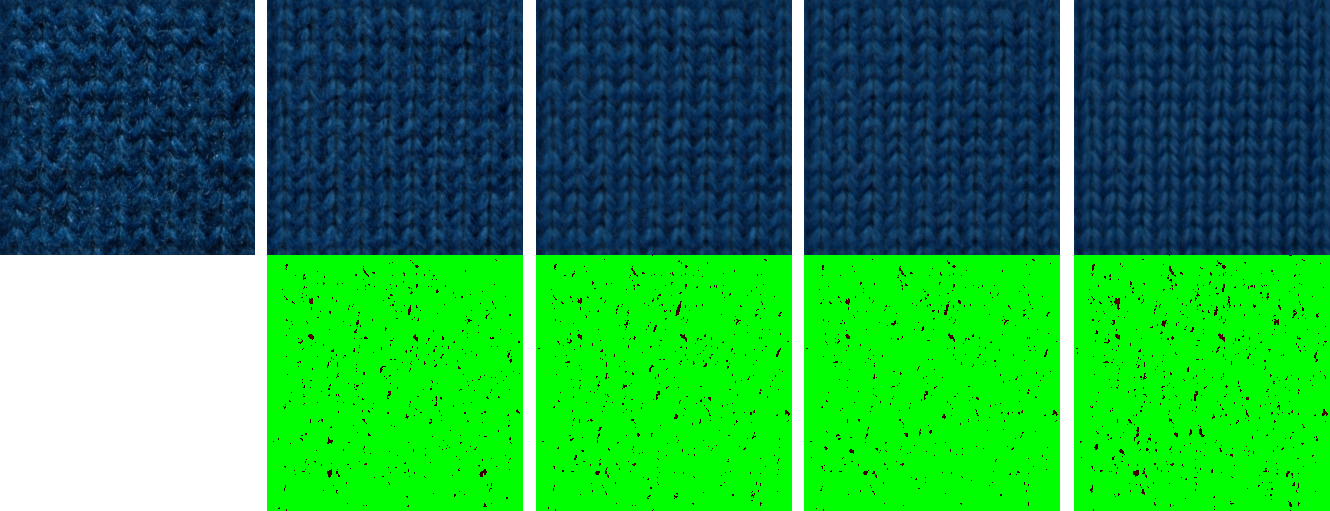
\includegraphics[width=1.0\textwidth]{figures/differ}
 \caption[Example of compression ] {
 	{\bf Example of compression \textnumero 2.}

	\textbf{First row} from the left to the right: original image, \textbf{32} components (RMSE:8.3\%), \textbf{16} components (RMSE:8.4\%), \textbf{8} components (RMSE:8.2\%), \textbf{4} components (RMSE:9.2\%). 
	\textbf{Second row}: the difference between original and decompressed, \emph{red} color denotes how big the error, \emph{green} denotes that error is absent or very small.}
 \label{fig:compression_example_2}
\end{figure}

\subsection{Decompression}
\label{section:Decompression}
The decompression step is simply matrix operations, which require to combine 3 matrices $U$, $\Sigma$, $V$ and mean vector $m$.
To make it a bit easier to decompress on GPU we construct new matrices as Borshukov et. al.

{\centering $L=\begin{bmatrix}
 m\mid U \Sigma
\end{bmatrix}$ \\}

{\centering $
R=\begin{bmatrix}
 1 ... 1   \\ 
  \, \, \, V^{T}
\end{bmatrix}.$ \\}
  Matrix $A$ takes such form of decompression $A=LR$. In detail, if want to decompress texture with index $i$ for first $C$ components, we do it separately for each color channel


{\centering $red(x,y)=\sum_{k=1}^{C}L_{xy,k}R_{k,3i+0}$ \\}
{\centering $green(x,y)=\sum_{k=1}^{C}L_{xy,k}R_{k,3i+1}$ \\}
{\centering $blue(x,y)=\sum_{k=1}^{C}L_{xy,k}R_{k,3i+2}$ \\}


\section{Viewing and Illumination Angle Interpolation}
\label{section:interpolation}

BTF datasets are measured for discrete number of angles, thus we would need to perform interpolation for unknown not measured angels.
We will employ barycentric coordinates interpolation. 
However, it is very computational heavy, so the following approximation algorithm proposed by Hatka and Haindl \cite{btfblender} will be used.

Assume that we have found triangle $P_{1}P_{2}P_{3}$ which bounds our point P, which we want to interpolate. Figure \ref{fig:acquisition_example} demonstrates hemisphere on which triangle $P_{1}P_{2}P_{3}$ lies.
$Y_{P}$ denotes desired pixel color. 
So, generally speaking linearly interpolation of that pixel will be $Y_{P}=w_{1}Y_{P1} + w_{2}Y_{P2} + w_{1}Y_{P2}$, 
where $Y_{P1},Y_{P2},Y_{P3}$ correspond to measured pixel color of positions $P_{1},P_{2},P_{3}$ accordingly. Weights $w_{1},w_{2},w_{3}$ are normalized and sum up to $1$.

Weights defined as volumes $V_{1},V_{2},V_{3}$ which correspond to $PP_{2}P_{3}O$, $PP_{3}P_{1}O$, $PP_{1}P_{2}O$ tetrahedrons, where $O=(0,0,0)$.
All volumes are normalized, which means $V_{i}=\frac{V_{i}}{\sum_{i=1}^{3}V_{i}}$. Volumes calculated as determinates of $4\times 4$ vectors

{\centering $V_{1}=\frac{1}{6}\left | det(PP_{2}P_{3}O) \right |$ \\}
{\centering $V_{2}=\frac{1}{6}\left | det(PP_{3}P_{1}O) \right |$ \\}
{\centering $V_{3}=\frac{1}{6}\left | det(PP_{1}P_{2}O) \right |$ \\}

\section{Streaming}
\label{section:streaming}


The size of compressed BTF data using PCA is around 10-20 Mb on a hard drive. 
Even though, compressed BTF data size is sufficient for plausible rendering, it is still big enough for transferring it over the internet for web rendering.
The full transfer of BTF may take some minutes, especially with slow internet connection. The solution to make this process faster and rendering a bit more interactive, we will use progressive streaming of BTF data.
Deploying streaming a user will be able to see a preview of original BTF in just in a few seconds. 
Principal components will be streamed one by one using WebSockets \cite{websockets}, and the rendering will be refreshed whenever a new component arrives.
The quality will be progressively improved during streaming, see Figure \ref{fig:streamPreview} for an example. Also, it is possible to show an overall progress for the user, which makes the process of streaming even more interactive.


We use WebSockets for streaming the data, as it is most efficient and elegant way of communicating between a server and a client.
The following advantages of WebSocket technology \cite[Ch.\ 1]{websockets}:

\begin{itemize}
  \item \textbf{Delivers high \emph{Performace}}  for real-time server-client connections. 
  Usually, web developers used well known methods such as polling, long polling, and HTTP streaming. However, WebSocket saves bandwidth, CPU power, and latency compared to those methods.
  For example, polling method makes requests to the server and has to wait for the response.
  With WebSockets the client does not need to wait for the response, because WebSockets reuse the same connection from client to the server and wise-verse.
  This single connection reduces the latency.

  \item \textbf{\emph{Saves time}} to develop web-applications. \emph{Simplicity} of is one of the main advantage over older methods for server-client communication.
  
\end{itemize}

\begin{figure}[h]
 \centering
 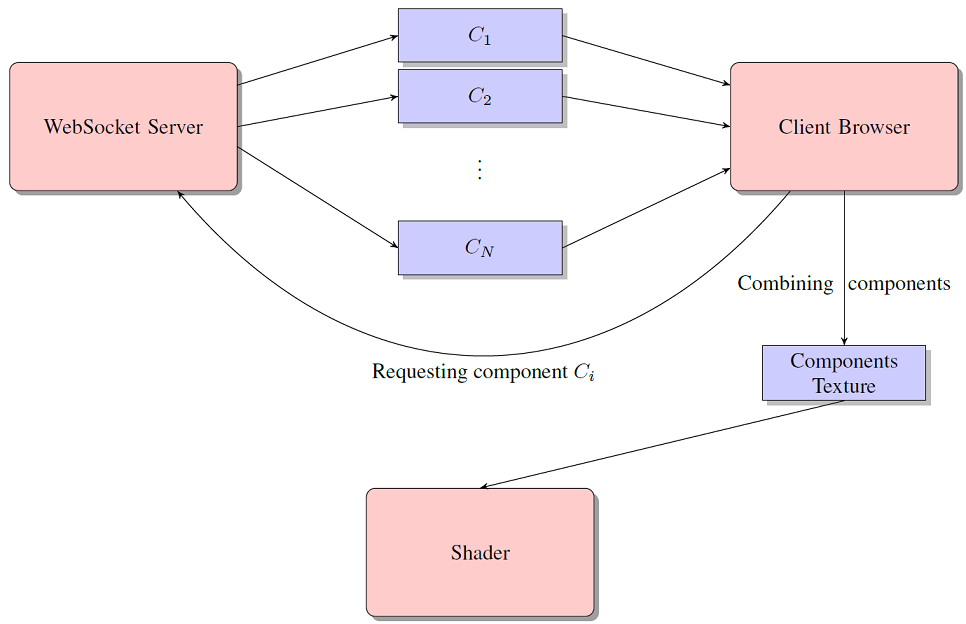
\includegraphics[width=1.0\textwidth]{figures/streaming}
 \caption[Streaming process illustration ] {
 	{\bf Streaming process illustration}
	}
 \label{fig:streaming}
\end{figure}


As it was described in Section \ref{section:algorithm_step} matrices $U$, $\Sigma$ and $V$ store all needed data to reconstruct BTF.
Matrices $\Sigma$ and $V$ are quite small in size, they are sent at first place. On the contrary, matrix $U$ stores principal components of size $W \times H$ which makes matrix $U$ the biggest in size of all.
On a client side before streaming, matrix $U$ is initialized with blank values, for example zeros. After a Socket connection was established, the client side requests one component at a time. 
Each new arrived component saved in matrix $U$ and the client side refreshes the shader to render BTF. Figure \ref{fig:streaming} illustrates this process.
 Also, each component is saved as PNG image on the WebSocket server, which makes a bit further compression of the BTF.

Consider Figure \ref{fig:streamPreview} that shows how the streaming works on practice.
We can see that even with first components the resulted texture looks quite decent.
With further components the overall quality of texture improves, e.g. specularities are increasing, small micro-structures become more visible and emphasized.
To make the streaming process a bit entertaining, the client also can see the progress-bar of the streaming progress.
Also, some of the mid-results were skipped in the Figure \ref{fig:streamPreview} for the sake of simplicity.

\begin{figure}[h]
 \centering
 \includegraphics[width=1.0\textwidth]{figures/streampreview}
 \caption[Example of Progressive Streaming ] {
 	{\bf Example of Progressive Streaming}

	\textbf{From left to right}: \emph{1}, \emph{2}, \emph{4}, \emph{6}, \emph{7}  components rendered at the same time.
	
	\textbf{Note}: \emph{8th} component is average grey value, which sends at first place.
	}
 \label{fig:streamPreview}
\end{figure}







\clearpage

\chapter{Implementation}

This chapter describes details, problems and limitations of the thesis implementation part.

The implementation of the demo-application is divided into three main parts: compression, streaming and rendering.
The compression is implemented as a standalone Java application, which compresses BTFs from the Bonn University \cite{btfBonn}.
It is possible to adapt any other BTF databases for our demo-application by resampling BTFs \cite{resampling}.
For streaming we use  Node.js \cite{nodejs} platform.
To integrate 3D graphics into HTML page we use XML3D \cite{xml3d}.
The overall model of the demo application is depicted in Figure \ref{fig:overview}.

\begin{figure}[h]
 \centering
 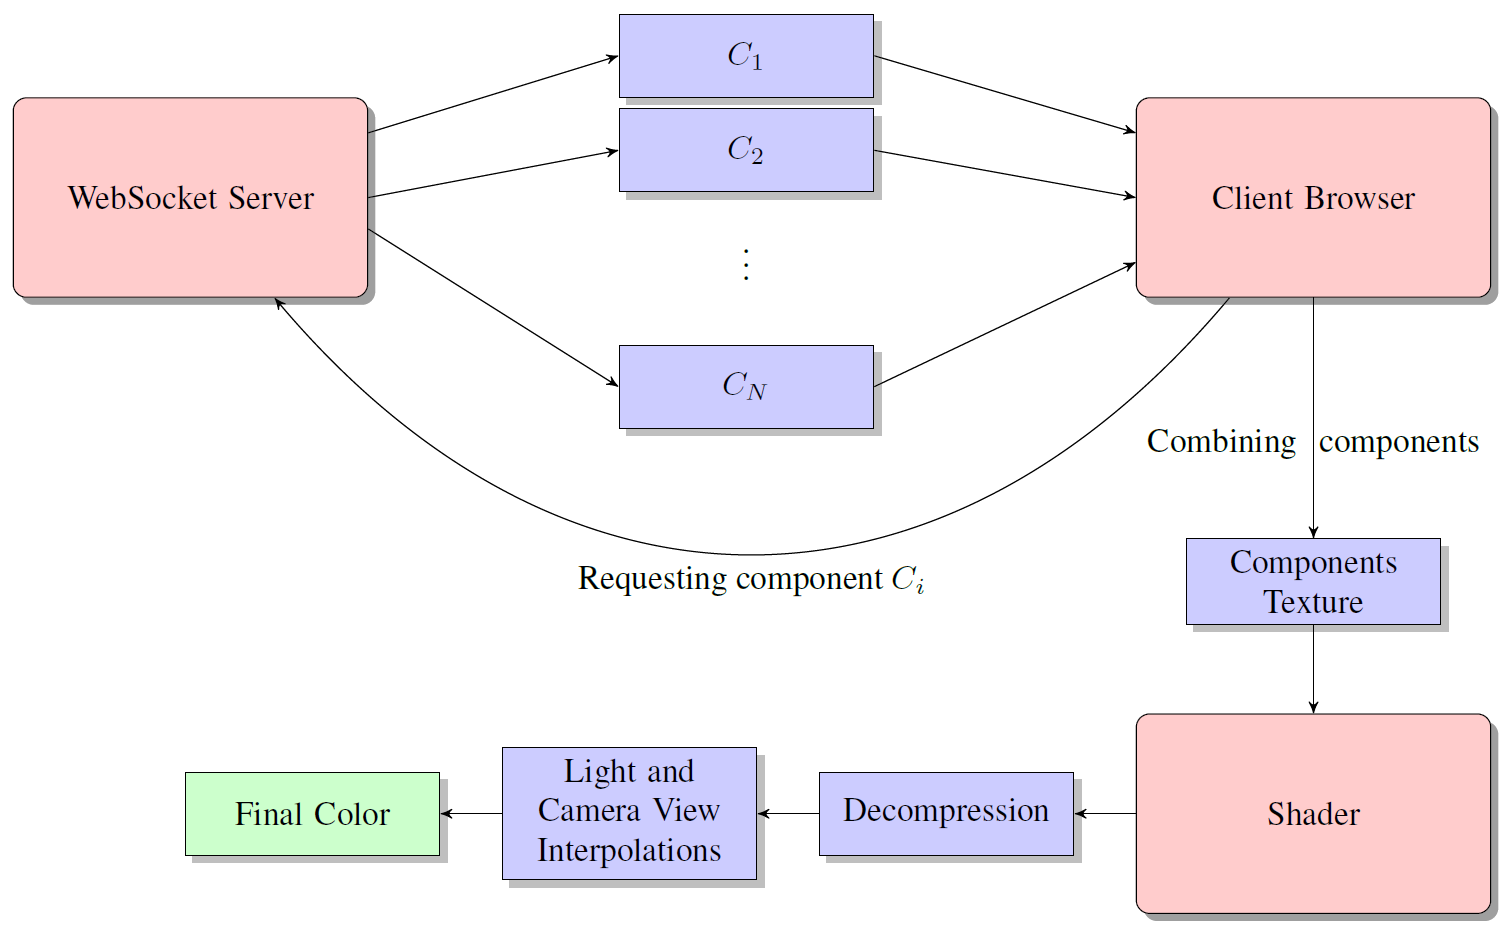
\includegraphics[width=1.0\textwidth]{figures/overview}
 \caption[Model Overview ] {
 	{\bf Model Overview}

	
	}
 \label{fig:overview}
\end{figure}



\section{Compression}
\label{section:impl_compression}

The implementation of the singular value decomposition (SVD) is the main part of the PCA implementation.
 We use \emph{jblas} \cite{jblas} library developed by Mikio Braun. 
 This is a linear algebra library written in Java language, which provides very high performance  \cite{jblas}.
 
The compressed BTFs  have to be sent to the shader. 
  OpenGL Shading Language (GLSL) version 1.0 support uniform arrays, however, they do not fully support dynamic indexing  \cite{glsl}.
Fortunately, it is possible to send arrays of data which are mapped to textures. 
After performing SVD, resulted matrices $U$, $\Sigma$, $V$ are saved as PNG images. (See Chapter \ref{chapter:implementation}).
Values of matrices $U$ and $V$ are in the range of $[-1;1]$.
 Those values have to be mapped to the image domain, i.e. $[0;1]$.
The following function is used to map the values:  

{\centering$f(x)=(x+1)/2$\\}


 Each component of the matrix $U$ is stored as the PNG image.
 For example, if compressed BTF data has $C$ principal components, then this would result in $C$ separate images.
 This is done for streaming purpose, so then principal components can be sent one by one from the server to the client.
 We use  RGBA color space to save four components into the one pixel, because it is possible to do efficient multiplication in the shader by using vector multiplications.
Matrices $V$ and $\Sigma$ are saved in the single shared texture, as they are small in size.

 The matrix $\Sigma$ is a diagonal matrix.
 The values of $\Sigma$ can be bigger than the image color value, i.e. an 8-bit value.
 In practice the values of $\Sigma$ for Bonn University BTFs \cite{btfBonn} are not bigger than four digit number $a_{4}a_{3}a_{2}a_{1}$.
We split the value into two values, i.e. 
 
{\centering$ \underbrace{a_{4}a_{3}}_{R} \underbrace{a_{2}a_{1}}_{G}$\\}
 
It means that two values of $\Sigma$ are mapped into the one pixel, i.e.  one value to RG  channels and the second to BA channels.
If the value of  $\Sigma$ exceed the four digit number, then it is possible to adapt this technique further in the similar manner.


We noticed that in case of Bonn Database \cite{btfBonn} the \emph{jblas} \cite{jblas} library produces relatively sparse values for $U$ and $V$, i.e. close to the zero.
 We scale the data to improve the floating point error caused by mapping of $U$ and $V$ back-and-forth.
The scaling improved the overall decompression error approximately by $5\%$.
 Using the following function we find the scaling factor:
 
 {\centering$ factor(M)=10^{floor(min[log10(min(M)),log10(max(M)]))}$ \\}
 
 where M is the matrix $U$ or $V$. The term $floor(min[log10(min(M)),log10(max(M))])$ calculates the degree with which it is possible to multiply the matrix and preserve the original values range, i.e. $[-1;1]$.
 If it is not possible, the resulting factor will be $1$.
As the decompression is computed as multiplication of $U\Sigma V$, we have to remain the original decompressed BTF values.
We do this by  multiplying each time $\Sigma$ values by the factor $\tfrac{1}{factor(M)}$ if we scale either $U$ or $V$.


 
\section{Streaming}
\label{section:impl_streaming}


We use Node.js \cite{nodejs} as a server side platform, which enables realtime streaming using WebSockets. On top of that, we use BinaryJS \cite{binaryjs} for the binary streaming.
BinaryJS is a framework that uses WebSockets to stream the binary data to the client from the Node.js server.
The server and the client applications are written in JavaScript.



\begin{figure}[h]
 \centering
 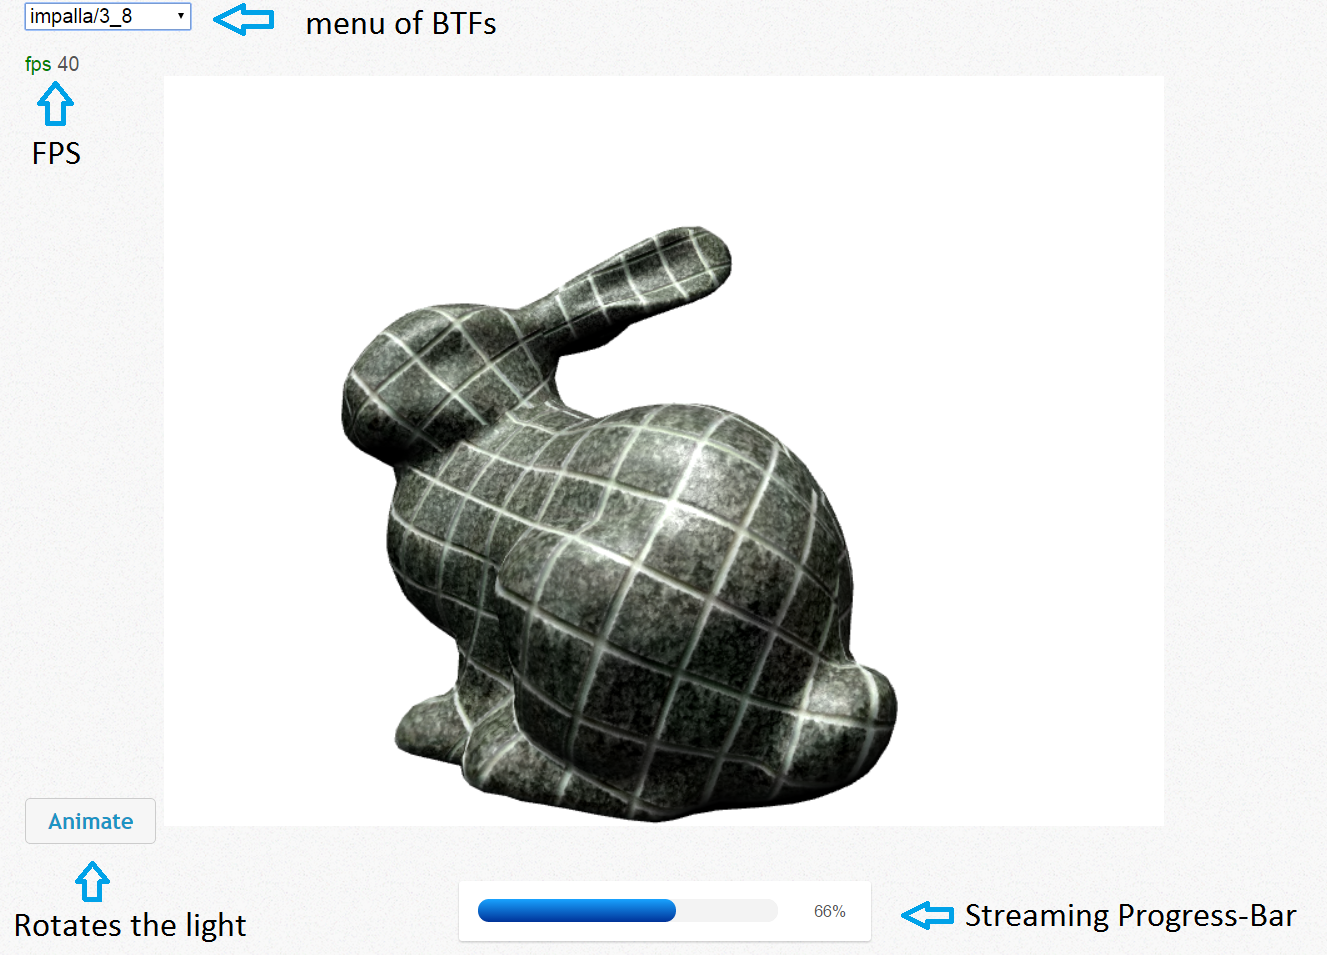
\includegraphics[width=1.0\textwidth]{figures/progress-bar}
 \caption[The streaming progress on the client side] {
 	{\bf The streaming progress on the client side }

 }
 \label{fig:progress-bar}
\end{figure}

We also use Xflow \cite{xflow}, which is a declarative language for data flow processing in realtime.
Xflow is a part of XML3D implementation. We use Xflow for gathering all the transferred principal components and storing them in one common texture $L$. (See Chapter  \ref{section:decompression}).

Consider Figure \ref{fig:streaming} from the Chapter \ref{chapter:streaming} that depicts how the streaming works on practice.
When the user connects to the streaming server and the HTML page loads completely, i.e. all the 3D objects are on the client side, the JavaScript client side sends the message to the Node.js server to start streaming the BTF data.
All the compressed BTFs are located on the Node.js server.
At the start of the stream, we first send texture $R$ and meta data. (See Chapter  \ref{section:decompression}).
Afterwards, each principal component $C_{i}$ are streamed in chunks one by one as PNG images.
Each $C_{i}$ covers all the angular domain, i.e. all the possible camera and light directions.

We decode PNG images using PNG decoder written by Arian Stolwijk \cite{pngreader}. PNG images are decoded to the array of RGB colors and saved to the common texture $L$ in canvas format using Xflow.
Each time the texture $L$ updates the rendering also refreshes.
Even with the first principal component the resulted image looks plausible.
With further components the overall quality of the image improves, i.e. specularities are increasing, small micro-structures become more visible and emphasized.
The user also  able to see the progress-bar of the streaming progress as shown in  Figure \ref{fig:progress-bar}.



Currently the limitation of such streaming approach is the drop of the frame rate when the assembling of the principal components occurs on the client side.
This is caused by the update of the canvas element (texture $L$) each time new component is transmitted to the client.
Also, we did not test the performance of multiple streaming, i.e. if there are several 3D objects that request BTFs at the same time.
 Our current implementation does not support this.
This can be included to the future work. 

\section{Rendering}
\label{section:impl_rendering}


We use XML3D \cite{xml3d} platform to embed 3D graphics into the HTML page. XML3D based on XML and allows for declaring your own 3D scenes and shaders.
XML3D is based on WebGL and JavaScript.

The shader design is depicted in Figure \ref{fig:shader}.
The compressed BTF data comes to the shader in the form of two textures. 
The first texture $L$ stores principal components and the second $R$ stores PCA weights. (See Chapter \ref{section:decompression}).
First, we find three closest directions for the camera and light directions. (See Chapter \ref{chapter:finding_triangle}).
Then, we compute barycentric coordinates for interpolation as described in Chapter \ref{chapter:barycentric}.

\begin{figure}[h]
 \centering
 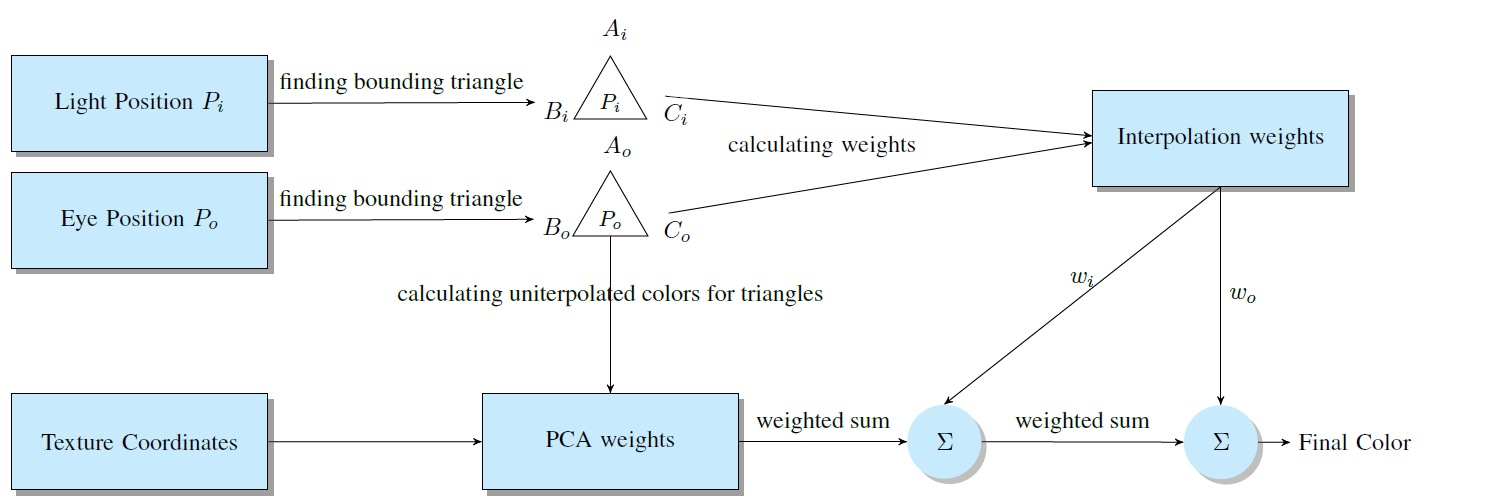
\includegraphics[width=1.0\textwidth]{figures/shader}
 \caption[Shader Design] {
 	{\bf Shader Design }

 }
 \label{fig:shader}
\end{figure}


In the next step we sample the input textures to decompress the needed values for found closest directions.
We have three closest directions per camera and light directions. This means for the interpolation we need to have nine color values. 
For a given texture coordinates $u,v$ we lookup the index of the first principal component, with which it will be possible to start the decompressing.
All the principal components are written linearly in texture $L$, i.e. one by one. 
We have the following mapping to get the needed index:

{\centering$indexL(i,j)= (b*N^2+ (i*N+j))*C$ \\}

where $i=\left \lfloor u*N\right \rfloor$, $j=\left \lfloor v*(N) \right \rfloor$, $b$ is the number of subsets, $N$ is the size of the compressed image and $C$ is number of components.
The parameter $b$ depends on the number of subsets on which PCA is separately done. (See Chapter \ref{section:algorithm_step}).

Texture $R$ stores PCA weights, we lookup the index of suitable compressed image.
The mapping depends on the camera direction $v=(\theta_v,\phi_v)$ and light direction $l=(\theta_l,\phi_l)$.
 It is defined as:

{\centering$ indexR(v,l)=offset(\theta_v,\phi_v)+offset(\theta_l,\phi_l)$\\}

where  $offset(\theta,\phi)=(\tfrac{\theta}{\Delta\theta}+\tfrac{\phi}{\Delta\phi})$, where $\Delta\theta$ and $\Delta\phi$ are quantization step sizes.

When all the indices are computed and textures L and R can be sampled, we decompress the colors as defined in Chapter \ref{section:decompression}.


In a final step we combine nine decompressed colors and early found interpolation weights to get the final color. (See Chapter \ref{chapter:interp_algo}).

The implemented shader has it's own limitations. First of all, the number of principal components has to be fixed for a shader, because GLSL version 1.0 does not allow for dynamic looping \cite{glsl}.
Secondly, the number of principal components are bound by a size of the texture $L$. It means that not all GPUs can handle very big textures. The problem can be fixed by using multiple textures.
But anyway these limitations does not directly influence the performance of the shader, which provides real-time frame rate and performs well even on the mobile devices. (See Figure \ref{fig:progress-bar}).






 




\clearpage

\chapter{Evaluation}
\label{chapter:Evaluation}
In this chapter we will evaluate the presented solution in regard to the decompression error, compression ratio and image quality and real-time performance during the streaming.


\section{Compression}
\label{section:eval_compression}


We evaluate our compression approach using the Bonn's BTF Database \cite{btfBonn} and compare the results to other related PCA methods \cite{haindl}.

We tested different configurations for the BTF compression and decided that the optimal configuration for our method is when $k=3$ and $C=8$, 
where $k$ is the number of neighbour directions and $C$ is the number of principal components. (See Chapter \ref{section:algorithm_step}).
Figure \ref{fig:compression_example} shows an example of the wool material decompressed with various number of components. The Mean Average Error (MAE) in CIELAB color space is computed for each of them.
The CIELAB metrics accounts for the human visual sensitivity, i.e. is consistent with human perception \cite{cielab}.
MAE is calculated for each of the channels separately and then the final result is averaged over them.

{\centering $MAE = \frac{1}{N}\sum_{i=1}^{N}(\left | y_i-\hat{y_i} \right |)$\\}

\begin{figure}[h]
 \centering
 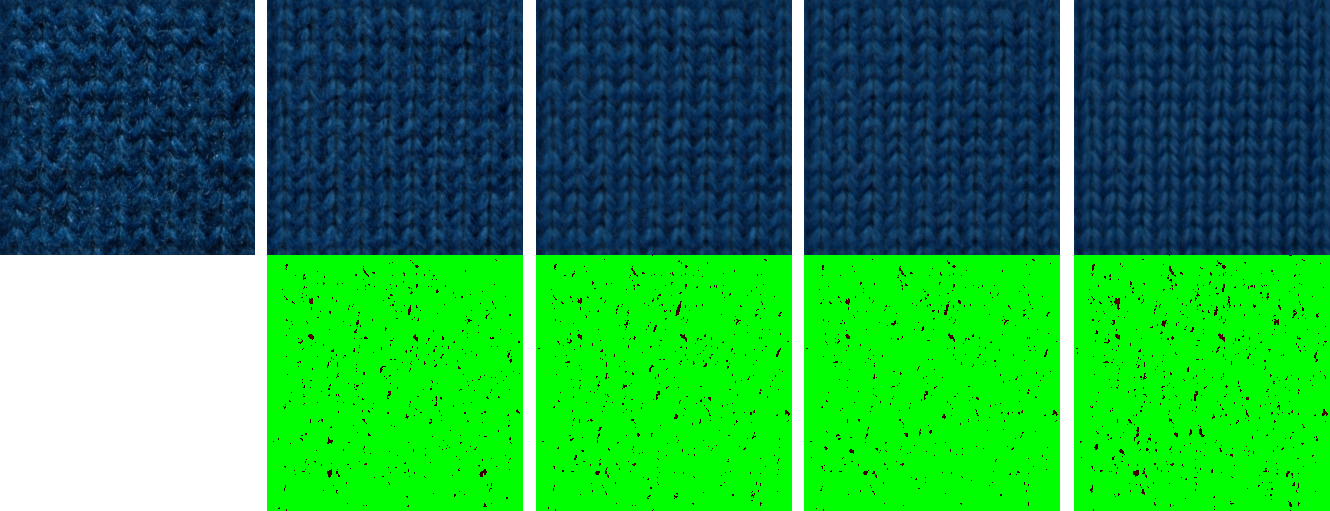
\includegraphics[width=1.0\textwidth]{figures/differ}
 \caption[Example of decompression errors ] {
 	{\bf Example of decompression errors }

	\textbf{First row} from the left to the right: ground truth, \textbf{32} components (MAE:2.17), \textbf{16} components (MAE:1.83), \textbf{8} components (MAE:2.21), \textbf{4} components (MAE:3.04). 
	\textbf{Second row}: the difference between the original and the decompressed images, \emph{red} color denotes how big the error, \emph{green} denotes that the error is absent or very small.}
 \label{fig:compression_example}
\end{figure}




 Figure \ref{fig:compression_example} shows that the decompression error is not significantly improved for $16$ or even $32$ components.
4 Components on the other hand result in a blurred image. This shows that our choice for 8 components is reasonable.
 Haindl \cite{haindl} also claims that $8$ components is the optimal number of components for the PCA RF method, which is related to our method.



 
\begin{table}[h]
\begin{tabular}{|l|l|l|c|c|c|c|c|}
\hline
     & k                      & C                      & \begin{tabular}[c]{@{}c@{}}MAE\\  CIELab\end{tabular} & \begin{tabular}[c]{@{}c@{}}MAE \\ RGB\end{tabular} & \begin{tabular}[c]{@{}c@{}}RMSE\\  RGB\end{tabular} & \multicolumn{1}{l|}{Compression Ratio} & \begin{tabular}[c]{@{}c@{}}Parameters Size /\\  Storage Size (PNGs)\end{tabular} \\ \hline
wool & \multicolumn{1}{c|}{1} & \multicolumn{1}{c|}{8} & 2.14                                                  & 5.86                                               & 7.5                                                 & 1:23                                   & 53Mb / 20 Mb                                                                     \\ \hline
wool & 3                      & \multicolumn{1}{c|}{8} & 2.19                                                  & 6.83                                               & 8.68                                                & 1:70                                   & 18Mb / 5Mb                                                                       \\ \hline
wool & 3                      & 32                     & 2.22                                                  & 5.92                                               & 7.5                                                 & 1:17                                   & 70Mb / 25Mb                                                                      \\ \hline
\end{tabular}
\caption{ Evaluation of BTFs}
\label{table:mytable}
\end{table}


 Table \ref{table:mytable} provides the evaluation for the whole BTF space of the wool sample, i.e. for all possible camera and light directions.
 The MAE is also computed in RGB color space along with the Root Mean Square Error to measure the variance in the errors
 
 {\centering $RMSE = \sqrt{\frac{1}{N}\sum_{i=1}^{N}(y_i-\hat{y_i} )^2}$\\}

 RMSE gives large weights to big errors, thus we can evaluate if big errors are present \cite{rmse}.
 The bigger the RMSE the bigger the variance of the errors. We can see that in our case the RMSE is close to the MAE, which means that the variance of the errors is relatively small.
 
In the first row of the  Table \ref{table:mytable} where $k=1$ our method becomes equal to the PCA RF \cite{haindl} method.
Haindl \cite{haindl} claims to have the MAE equal to $3.16$ in CIELAB color space for the same sample.
 Our method produces better result, i.e. $2.14$. 
 The second row shows that for  $k=3$ MAE stays practically the same. 
 However, the compression ratio improves by a factor of three.
 We can see that even for $32$ components the decompression errors improves only insignificantly, but the compression ratio becomes worse.
 If we use $k>3$, more components would be necessary to reduce decompression errors.
 For intance, our method becomes equal to the PCA BTF \cite{haindl} method if $k=81$ (all camera directions). 
 In this case approximately $41$ components are necessary \cite{haindl}.
 
 Also, the LPCA BTF \cite{haindl} method uses $19$ components on average and has the MAE equal to $2.42$, while our method uses $8$ components.
 
 

\section{Real-time performance}
\label{section:eval_streaming}


We evaluate the rendering quality during the streaming and the real-time performance.
Figure \ref{fig:streamPreview} depicts intermediate images during the streaming.
We tested our approach on three materials: wool, impalla and corduroy.
The parameters for the compression are $k=3$ and $C=8$.

\begin{figure}[h]
 \centering
 \includegraphics[width=.87\textwidth]{figures/streampreview}
 \caption[Example of Progressive Streaming ] {
 	{\bf Example of Progressive Streaming}

	\textbf{From left to right}: \emph{1}, \emph{2}, \emph{4}, \emph{6}, \emph{8}  components rendered accordingly.
	}
 \label{fig:streamPreview}
\end{figure}
\label{chapter:implementation}



\begin{figure}[h]
 \centering
 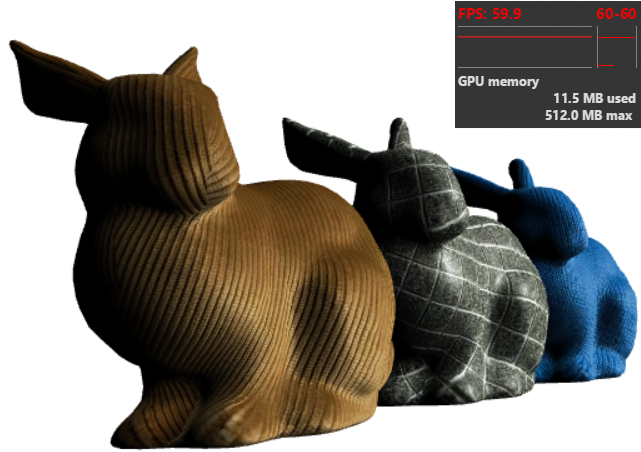
\includegraphics[width=.65\textwidth]{figures/3BTFs}
 \caption[Example of 3 BTFs rendered at the same time ] {
 	{\bf Example of 3 BTFs rendered at the same time }

	\textbf{From left to right}: corduroy, impalla and wool materials are rendered under dynamic light.
	}
 \label{fig:3BTFs}
\end{figure}
\label{chapter:implementation}

Rendering starts as soon as the first component transfers to the client side.
 The overall appearance of the the material is already visible even with the first the component, which has an average size of about $0.7$Mb.
With further components the overall quality of the image improves, i.e. specularities are increasing, small micro-structures become more visible and emphasized.
On a desktop computer with a NVIDIA GeForce GTX 480 graphics card 3 BTFs can be rendered at 60 frames per second.
Figure \ref{fig:3BTFs} shows an example of this.

On a Sony Xperia SL 15 frames per second are achieved on average for one BTF at a time.


\section{Comparison with the Phong Shader}
\label{section:eval_streaming}

Figure \ref{fig:phongvsbtf} shows the tremendous difference between the BTF and a conventional 2-D texture in combination with the Phong shader.
Both images were taken under the same camera and light directions. The BTF introduces high varying specularities and the realistic depth in the images.
The Phong shader with the combination of the 2-D texture provides the impression that the material looks flat.
The BTF shows the correct inner-reflections, sub-surface scattering and shadows under varying light conditions.

\begin{figure}[hb]
 \centering
 \includegraphics[width=.73\textwidth]{figures/phongVsBTF}
 \caption[The Phong model in comparison to the BTF ] {
 	{\bf The Phong model in comparison to the BTF  }
	}
 \label{fig:phongvsbtf}
\end{figure}


\clearpage

\chapter{Conclusions and Future Work}
\label{chapter:conclusions}
 Bidirectional Texture Functions are currently the best texture representation for the materials 
 that contain high frequencies both in the angular and spatial domain \cite{mueller-2003-compression}.
 Thousands of images has to be taken to sample the appearance of such materials.
 Due to huge sizes of acquired BTFs real-time rendering is impossible to achieve without suitable compression.
 Thus, BTFs still staying in a state of the art in computer graphics. 

\section{Summary}

 In this work we achieved real-time rendering of BTFs in a high quality.
 Considering that we render BTFs in a browser, we managed to reduce the latency that is caused by the data transmission, i.e.
 by streaming  principal components individually.
 We are able to show immediately intermediate rendering results of the textured 3D object.
 We showed experimentally that it is possible to improve the decompression error that was caused by floating point imprecisions.
 The scaling of the compressed BTF data before converting it into the textures improved the decompression error approximately by $5\%$.
 As a result this also improved the real-time frame rates and the compression ratio due to reduction in the number of components used.


Finally, our method is flexible and allows for balancing between the visual quality, memory usage and computational effort.
\section{Future work}
\label{section:future_work}

Based on our results several directions for the future work can be made.
First of all, multiple streaming of BTFs can be implemented.
Secondly, several optimizations of the BTF shader performance can be made.
For instance, it is possible to reduce some of the calculations such as computation of the interpolation weights. 
They can be precomputed and stored in a cube-map \cite{haindl}.
Other calculations such as computation of the bidirectional normals can be precomputed and stored along with a 3D mesh.

Last but not least, there is a room for further compression.
 For instance, it can be achieved by compressing the PCA parameters with wavelet compression \cite{webglbtfstreaming} or with entropy encoding \cite{gpu_gems}. 
However, the decompression cost will grow, but it can be worth if further memory savings are necessary. 
\clearpage


% *************** Bibliography ***************
\bibliographystyle{plain}
{\small\bibliography{references}}
\clearpage



% *************** Back matter ***************
%\backmatter
%\input{back.tex}

\end{document}